\documentclass[conference]{IEEEtran}
\IEEEoverridecommandlockouts
% The preceding line is only needed to identify funding in the first footnote. If that is unneeded, please comment it out.
\usepackage{cite}
\usepackage{amsmath,amssymb,amsfonts}
\usepackage{algorithmic}
\usepackage{graphicx}
\usepackage{textcomp}
\usepackage{xcolor}
\usepackage{enumitem}
\usepackage{physics}
\def\BibTeX{{\rm B\kern-.05em{\sc i\kern-.025em b}\kern-.08em
    T\kern-.1667em\lower.7ex\hbox{E}\kern-.125emX}}
\begin{document}

\title{Recunoastere pe baza de semnaturi\\
{\footnotesize \textsuperscript{*}Procesare de Imagini - 9 Mai 2019}
}

\author{\IEEEauthorblockN{Catalin Moldovan}
\IEEEauthorblockA{\textit{Grupa 30235} \\
Universitatea Tehnica din Cluj-Napoca \\
catalin.moldovan@student.utcluj.ro}
}

\maketitle

\begin{abstract}
Acest document descrie doi algoritmi eficienti ce poat fi utilizat pentru verificarea semnaturii unei persoane. Metoda partitionarii imaginilor de test prin histograma cu un numar de acumulatori redus si algoritmul de clasificare Kmeas pe baza de SVM. Algoritmul poate fi utilizat in diferite companii, banci, pentru validarea documentelor si a contractelor.
\end{abstract}

\begin{IEEEkeywords}
Preprocesare, Thresholding, Histograma, KNN, K-means, Detectarea varfurilor, Distanta Euclidiana
\end{IEEEkeywords}

\section{Introducere}
Semnatura reprezinta o metoda de identificare a unei persoane, ce contine diferite caractere ce nu pot fi intotdeauna citibile. Prin evolutia tehnologiei, a evoluat in acelasi timp si modul de verificare a semnaturii unei persoane, crescand probabilitatea de recunoastere. Analiza unei semnaturii pe baza unei imagini se efectueaza ca imagine intreaga si nu ca litere si cifre puse impreuna. Biometria face referire la autentificarea unei persoane in functie de factori psihologici si comportamentali. Aceasta face diferenta dintre dintre indivizi. In aceasta lucrare se va pune problema pe biometria scrisului si reprezentarea unei metode de verificare a semnaturii folosind procesare de imagini. Pentru verificarea unei semnaturi, se vor utiliza un set de semnaturi obtinute de catre posesor in trecut. Prin efectuarea unor comparari a unor factori, se valideaza integritatea semnaturii. 

\subsection{Metode de verificare}
Verificarea unei semnaturi poate fi impartita in doua categorii: online si offline.

\paragraph{Online}
Verificarea semnaturii online reprezinta o metoda de recunoastere a scrisului in decursul scrierii. Exista diferiti factori, precum timpul petrecut cu varful pixului pe suprafata, forta de apasare, etc. Se pot extrage diferite elemente ce pot caracteriza posesorul semnaturii. Aceasta metoda duce la o acuratete ma buna, deoarece perceptiile emotionale si de presiune sunt foarte greu de imitat. 

\paragraph{Offline}
In cazul semnaturilor offline este necesara scanarea imaginii sau fotografierea ei, iar apoi folosirea unei aplicatii digitale pentru detectarea autenticitatii.

\section{Metode de verificare}
O metoda de identificarea a semnaturii este antrenarea sistemului cu un numar de 6 semnaturi de test, pe baza algoritmului ``Backpropagation`` \cite{b1}.

O alta metoda de identificare este printr-un proces de detectie a varfurilor prin algoritmul Canny (Sectiunea \ref{sec:Canny}). In final se va folosi distanta Eclidiana (Sectiunea \ref{sec:K-nearest}) pentru clasificarea imaginii cu cele de test \cite{b2}.

\section{Identificarea semnaturii}

\subsection{Preprocesarea imaginii}
Pasii necesari pentru transformarea unei imagini sub o forma convenabila sunt urmatorii:
\begin{itemize}
	\item imagine grayscale
	\item binarizare imagine
	\item decupare imagine
	\item normalizare imagine
\end{itemize}
\begin{figure}[h!]
	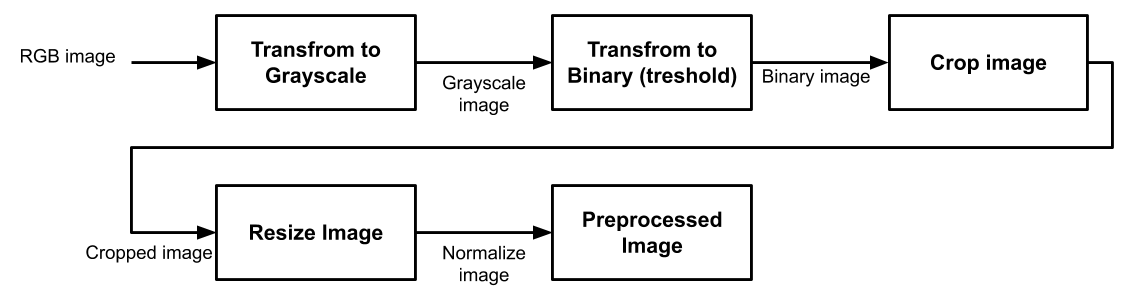
\includegraphics[width=\linewidth]{Figures/TransformationProcess.png}
	\caption{Pasi preprocesare}
	\label{fig:TransformationProcess}
\end{figure}

Primul pas reprezinta conversia imaginii RGB intr-o imagine grayscale. Prin acest proces se va reduce complexitatea si timpul de executie al sitemului. Este mult mai usor de executat operatii pe o imagine alb-negru, decat pe o imagine color. Este necesar un proces de binarizare a imaginii pentru indepartarea zgomotului. Urmatorul pas este reprezentat de un algoritm de decupare. Decuparea consista in separarea regiunii de interes fata de imaginea completa. Prin aceasta se vor indeparta pixelii albi, ceea ce va reduce mai mult timpul de procesare.

\begin{figure}[h!]
	\centering
	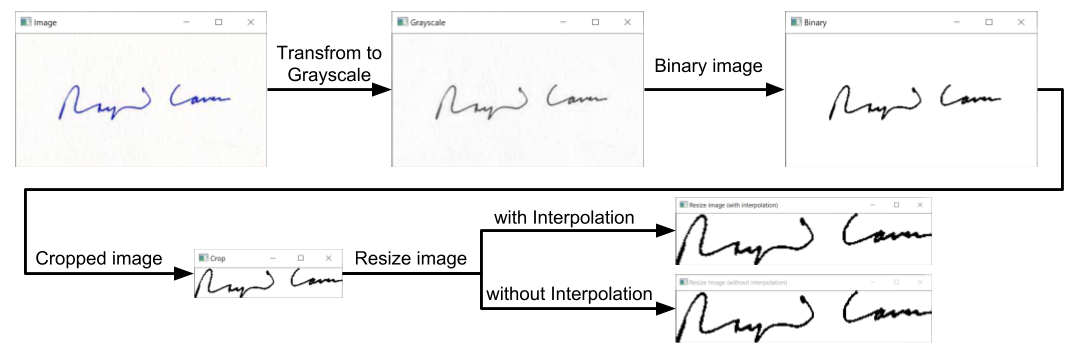
\includegraphics[width=\linewidth]{Figures/TransformationEg.png}
	\caption{Preprocesare imagine}
	\label{fig:Transformation}
\end{figure}

$\newline$

Normalizarea semnaturii va elimina diferentele de marimi a imaginii curente pentru a corespunde exact cu semnaturile de test din baza de date. Astfel pentru diverse comparatii, rezultatele vor fi mai usor vizibile, Fig. \ref{fig:Transformation}.



\subsection{Propunerea sistemului}
Diagrama bloc propusa sistemului este prezentata in Fig. \ref{fig:DiagramaBloc}.
\begin{figure}[h!]
	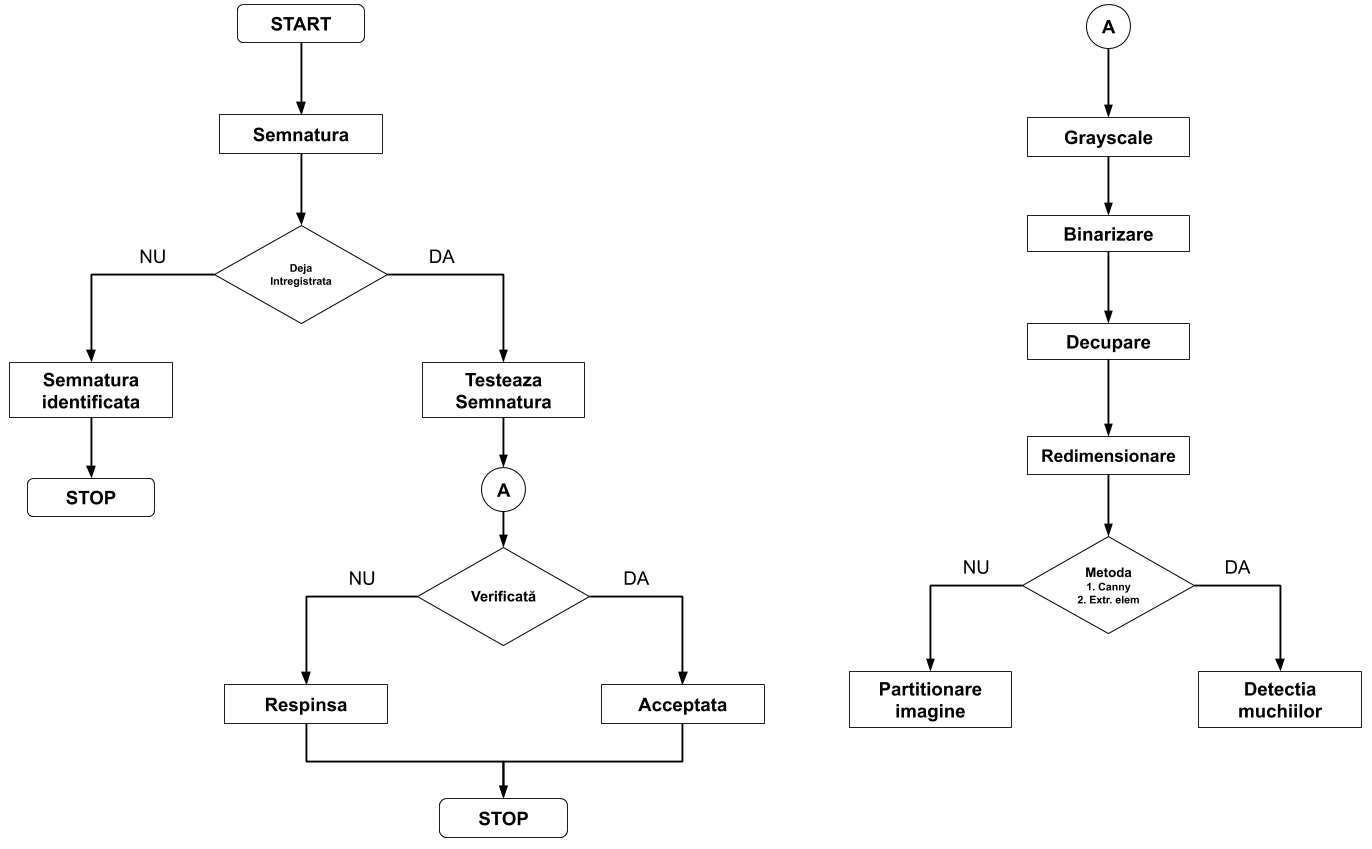
\includegraphics[width=\linewidth]{Figures/DiagramaBloc.png}
	\caption{Diagrama Bloc}
	\label{fig:DiagramaBloc}
\end{figure}

\section{Metoda partitionarii}
\subsection{Extragerea elementelor}
O metoda de verificare a semnaturii este compararea anumitor elemente ce tin de numarul de pixeli pe orizontala si verticala a imaginii decupate. Imaginea decupata va duce la eliminarea diferitelor proportii ale semnaturii. In functie de calitatea imaginii, aceasta este impartita intr-un numar redus de acumulatoare, Fig. \ref{fig:SignatureProcess}.

\begin{figure}[h!]
	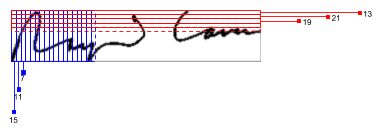
\includegraphics[width=\linewidth]{Figures/SignatureProcess.png}
	\caption{Partitionare semnatura}
	\label{fig:SignatureProcess}
\end{figure}

Dupa finalizarea parcurgerii imaginii, putem concepe o histograma bazata pe numarul de pixeli pe orizontala si pe verticala a imaginii decupate, impartind lungimea si inaltimea imaginii in \textit{m}, repsectiv \textit{n} parti egale, iar apoi sa numaram pixelii care apartin fiecarei parti, Fig. \ref{fig:Histograma}.

\begin{equation}
H(height)=N_{h}, h \in [0...m]\label{eq}
\end{equation}
\begin{equation}
H(width)=N_{w}, w \in [0...n]\label{eq}
\end{equation}

\begin{figure}[h!]
	\centering
	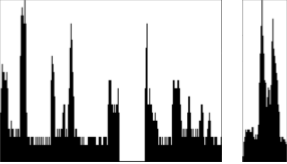
\includegraphics[scale=0.55]{Figures/Histograma.png}
	\caption{Histograma pixeli pe orizontala si verticala}
	\label{fig:Histograma}
\end{figure}

\subsection{Clasificare}
Aceasta sectiune prezinta modul de identificare a semnaturii persoanei. Se vor efectua comparatii succesive a numarului de pixeli pe orizontala si verticala a imaginii decupate cu cele de test. Pentru fiecare comparatie cu o imagine de test va rezulta o probabilitate, ce semnifica rata de identificare a posesorului semnaturii. Media probabilitatilor fiecarui set de semnaturi de test, respectiv probabilitatea cea mai ridicata si cu un procent mai mare de 60\%, va reprezenta o potrivire a semnaturilor. Un exemplu este prezentat in Tabelul \ref{Probabilitati}.

\begin{table}[h!]
	\caption{SET DE PROBABILITATI}
	\begin{center}
		\begin{tabular}{|c|c|c|c|}
			\hline
			\textbf{Probabilitate}&\multicolumn{3}{|c|}{\textbf{Comparare semnaturi baza de date}} \\
			\cline{2-4} 
			\textbf{Imagine} & \textbf{\textit{Prob. Test 1}}& \textbf{\textit{Prob. Test 2}}& \textbf{\textit{Prob. Test 3}} \\
			\hline
			65\% & 45\% & 76\% & 57\% \\
			25\% & 24\% & 36\% & 17\% \\
			82\%$^{\mathrm{*}}$ & 75\% & 91\% & 88\% \\
			34\% & 33\% & 45\% & 27\% \\
			\hline
			\multicolumn{4}{l}{$^{\mathrm{*}}$Setul de imagini cu probabilitatea cea mai ridicata.}
		\end{tabular}
		\label{Probabilitati}
	\end{center}
\end{table}

\section{Metoda Canny} \label{sec:Canny}
Metoda Canny se bazeaza pe calculul gradientului imaginii si in plus permite maximizarea raportului semnal zgomot pentru o detectie corecta, o localizare buna a punctelor de muchie si minimizarea numarului de raspunsuri pozitive la o singura muchie singulara, Fig. \ref{fig:Canny}.

Pasii metodei Canny \cite{b3}:
\begin{enumerate}[label=\Alph*.]
	\item Filtrarea imaginii cu un filtru Gaussian pentru eliminarea zgomotelor.
	\item Calculul modulului si directiei gradientului.
	\item Suprimarea non-maximelor modulului gradientului.
	\item Binarizarea adaptiva a punctelor de muchie si prelungirea muchiilor prin histereza.
\end{enumerate}

\subsection{Filtrarea imaginii cu un filtru Gaussian}
Zgomotul din imagine este o informație de “frecventa inalta” care se suprapune peste imaginea originala. Aceasta inducea aparitia unor puncte de muchie false. Zgomotul inerent procesului de achizitie al imaginilor are un model Gaussian si se poate elimina cu un filtru omonim.

\subsection{Calculul modulului si directiei gradientului}
Calcularea modulului gradientului (Ecuatia \ref{eq:Gradient}) si directiei gradientului (Ecuatia \ref{eq:Directia}) presupune alocarea a câte unui buffer temporar de dimensiunea imaginii și inițializarea elementelor lor.

\begin{equation} \label{eq:Gradient}
\abs{\triangledown f(x,y)} = \sqrt{(\triangledown f_{x}(x,y))^2 + (\triangledown f_{y}(x,y))^2}
\end{equation}

\begin{equation} \label{eq:Directia}
\theta(x,y) = arctg(\frac{\triangledown f_{y}(x,y)}{\triangledown f_{x}(x,y)})
\end{equation}

Componentele orizontale $\triangledown$f$_{x}$(x,y) si respectiv verticale $\triangledown$f$_{y}$(x,y) se calculeaza prin convolutia imaginii prin nucleul Sobel (Ecuatia \ref{eq:Sobel}).

\begin{equation} \label{eq:Sobel}
	\triangledown f_{x} = f(x,y)*	
	\begin{bmatrix}
		-1 & 0 & 1\\
		-2 & 0 & 2\\
		-1 & 0 & 1\\
	\end{bmatrix}
\end{equation}

\subsection{Suprimarea non-maximelor modulului gradientului}
Suprimarea are drept scop subtierea muchiilor prin pastrarea doar a punctelor de muchie care au modulul maxim al gradientului de-a lungul directiei de variatie a intensitatii, de-a lungul directiei gradientului. Astfel se cuantifica directile gradientului in 4 intervale de câte 45$^\circ$. In final se obtine o imagine in care intensitatea pixelilor este egala cu valoarea modulului gradientului in acel punct.

\subsection{Binarizarea adaptiva a punctelor de muchie si prelungirea muchiilor prin histereza}
\paragraph{Binarizarea adaptiva} 
Incearca sa extraga un numar relativ constant de puncte de muchie pentru o dimensiune data a imaginii. In acest fel se compenseaza iluminarea si contrastul diferit intre imagini. (Ecuatia \ref{eq:Binarizare}), unde parametrul p ia valori intre 0.01 și 0.1.Totusi nu garanteaza completitudinea muchiilor, deoarece anumite parti umbrite ale obiectului sau prezenta zgomotelor pot afecta procesul de detectie. Rezultatul va fi o imagine cu foarte multe muchii fragmentate.

\begin{equation} \label{eq:Binarizare}
NrPctMuchie = p * (NrPixeli - NrPixeliGradNul)
\end{equation}

\begin{figure}[h!]
	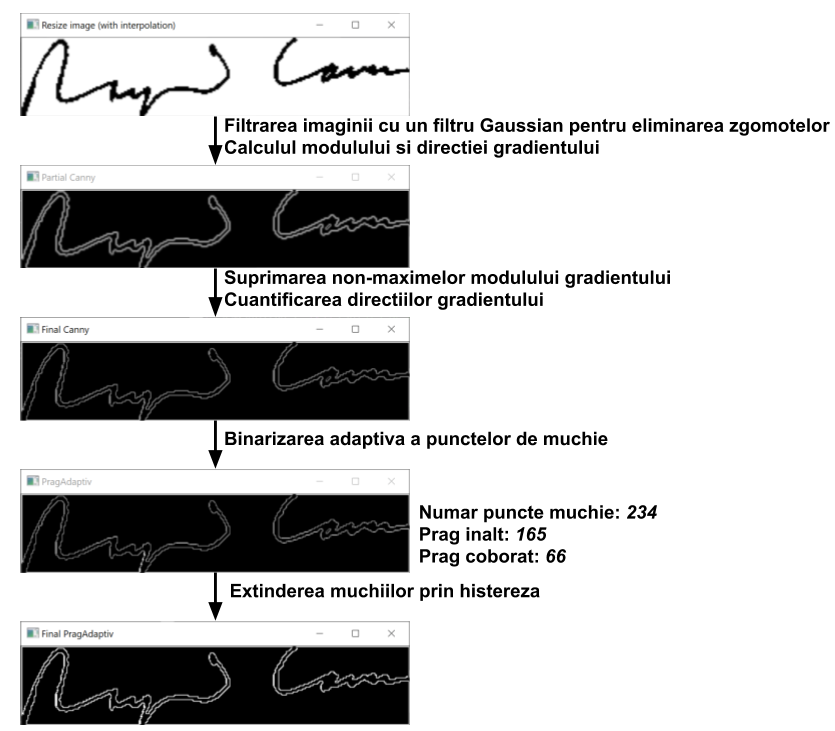
\includegraphics[width=\linewidth]{Figures/Canny.png}
	\caption{Detectia punctelor de muchie}
	\label{fig:Canny}
\end{figure}

Algoritm:
\begin{enumerate}
	\item Se calculeaza histograma de intensitati a imaginii.
	\item Se calculeaza numarul de pixeli diferiti de zero care nu vor fi puncte de muchie.
	\item Gasim valoarea intensitatii sub care se gasesc numarul de non muchii pixeli.
\end{enumerate}

\paragraph{Extinderea muchiilor prin histereza} 
Se impune o tehnica de prelungire a muchiilor. Muchiile obtinute prin binarizarea initiala se cauta a se prelungi cu muchii mai putin clare, care nu trec testul binarizarii cu acest prag, dar ar putea sa apara ca muchii la un prag mai scazut.

\section{K-nearest neighbours} \label{sec:K-nearest}
KNN este o metoda de clasificare bazata pe instante. Algoritmul pesupune ca imaginea este plasata intr-un spatiu n-dimensional. Fiecare instanta de test este clasificata in functie de cele mai apropiate k exemple din imaginile de test, fara a incerca sa se determine functia de distributie pe baza careia instantele sunt plasate in spatiul n-dimensional \cite{b4}.

Pentru a gasi si extrage din exemplele de test, este nevoie de o metoda de a compara cat de similare sunt doua instante. Pentru aceasta se foloseste distanta euclidiana. Urmatorul pas este sa se calculeze distanta dintre imagine si toate exemplele de test. In ultimul pas se determina care sunt cele mai apropiate k instante din setul de imagini de test si pe baza acestor instante similare se decide care este cea mai probabila clasificare a acesteia. Acest lucru se realizeaza prin votarea intre cele mai similare k instante, Fig. \ref{fig:KNN} \cite{b5}.

\begin{figure}[h!]
	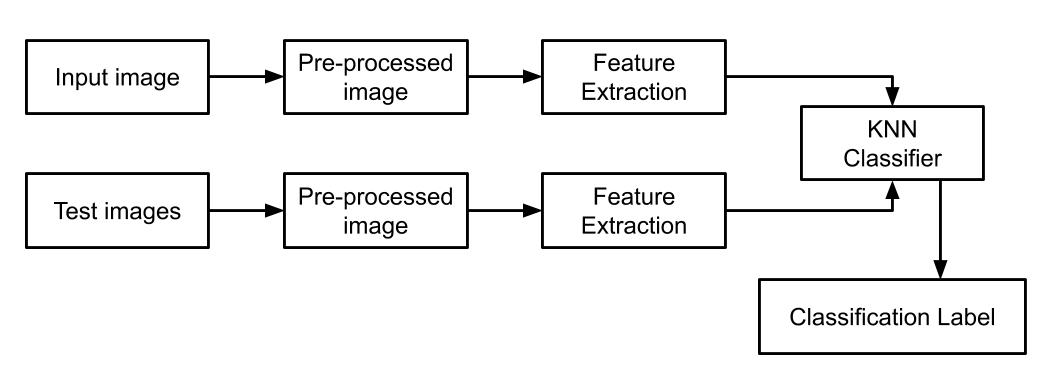
\includegraphics[width=\linewidth]{Figures/KNN.png}
	\caption{Diagrama bloc a metodei propuse utilizand KNN}
	\label{fig:KNN}
\end{figure}

\subsection{Distanta Euclidiana}
Distanta euclidiana reprezinta distanta geometrica intre doua puncte in spatiul bidimensional definita ca linia dreapta care le uneste (Ecuatia \ref{eq:DistantaEuclidiana}). In alte cuvinte, reprezinta distanta dintre doua puncte ce poate fi masurata cu un liniar. Aceasta este data de teorema lui Pitagora.

Folosind aceasta formula ca distanta, spatiul euclidian devine spatiu metric. Astfel putem genera valori exacte prin potrivirea imaginii date cu semnaturile de test \cite{b6}.

\begin{equation} \label{eq:DistantaEuclidiana}
d_{E}(P_{1},P_{2}) = \sqrt{(x_{1}-x_{2})^2 + (y_{1}-y_{2})^2} = \abs{\abs{P_{1}-P_{2}}}
\end{equation}

%https://www.academia.edu/27769393/Offline_Signature_Verification_based_on_Euclidean_distance_using_Support_Vector_Machine

\section{K-means}
Pentru compararea imaginilor de test cu cea de intrarem se va folosi un algoritm de clasificare a celor mai apropiati vecini, apoi vom trece la clasificarea liniara utilizand SVM (support vector machines). Algoritmul `bag of words` va realiza o clasificare bazata pe histograma de frecventa a anumitor caracteristici. Astfel se vor compara detectori, Laplacian, descriptori si functii kerneli SVM, Fig. \ref{fig:Kmeans}. \cite{b7}

\begin{figure}[h!]
	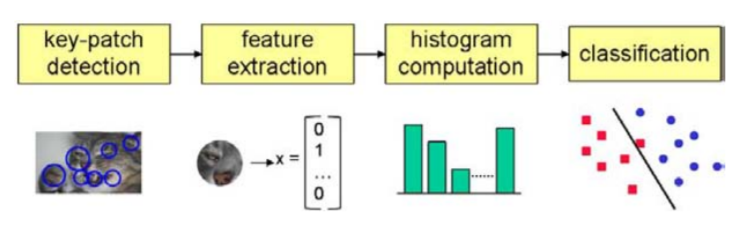
\includegraphics[width=\linewidth]{Figures/Kmeans.png}
	\caption{Procesul de clasificare K-means}
	\label{fig:Kmeans}
\end{figure}

Pentru estimarea distantei functiei kernel, se va forma o \textit{imagine de semnatura} (Ecuatia \ref{eq:DistanceKernel}).

\begin{equation} \label{eq:DistanceKernel}
S=((t_{1},\textbf{m}_{1}),...,(t_{m},\textbf{m}_{m}))
\end{equation}

Urmatorul pas reprezinta investigarea a doi kerneli diferiti pentru compararea \textit{imaginii de semnatura} prin EMD (earth mover's distance) (Ecuatia \ref{eq:EarthMoversDistance}), unde $f_{ij}$ reprezinta fluxul si $d(\textbf{m}_{i},\textbf{m'}_{j})$ distanta Euclidiana (Ecuatia \ref{eq:DistantaEuclidiana}).

\begin{equation} \label{eq:EarthMoversDistance}
EMD(S,S')=\frac{\sum_{i}\sum_{j}f_{ij}d(\textbf{m}_{i},\textbf{m'}_{j})}{\sum_{i}\sum_{j}f_{ij}}
\end{equation}

A doua distanta calculata va masura modul in care doua semnaturi au fost generate prin procesul de consistenta intamplatoare, apoi aceasta fiind convertita in kernel SVM folosind un kernel Gausian (Ecuatia \ref{eq:GaussianKernel}), unde A reprezinta parametrul de scalare stabilit la deistanta medie dintre imaginile de antrenament.

\begin{equation} \label{eq:GaussianKernel}
K(S,S')=exp(-\frac{1}{A}D(S,S'))
\end{equation}

Imaginile de test vor fi impartite in categorii unice, fiecare categorie reprezentand un individ, avand un anumit numar de semnaturi de test pentru antrenarea programului. In functie de descriptorii extrasi din fiecare imagine se vor compara imaginilie prin algoritmul de grupare K-means. \cite{b8}

Scopul metodelor de grupare (clusterizare) este de a partitiona o multime de obiecte in grupuri diferite, unde instantele dintr-un grup sunt similare intr-un anumit sens, Fig. \ref{fig:DescriptoriSemnatura}. 

\begin{figure}[h!]
	\centering
	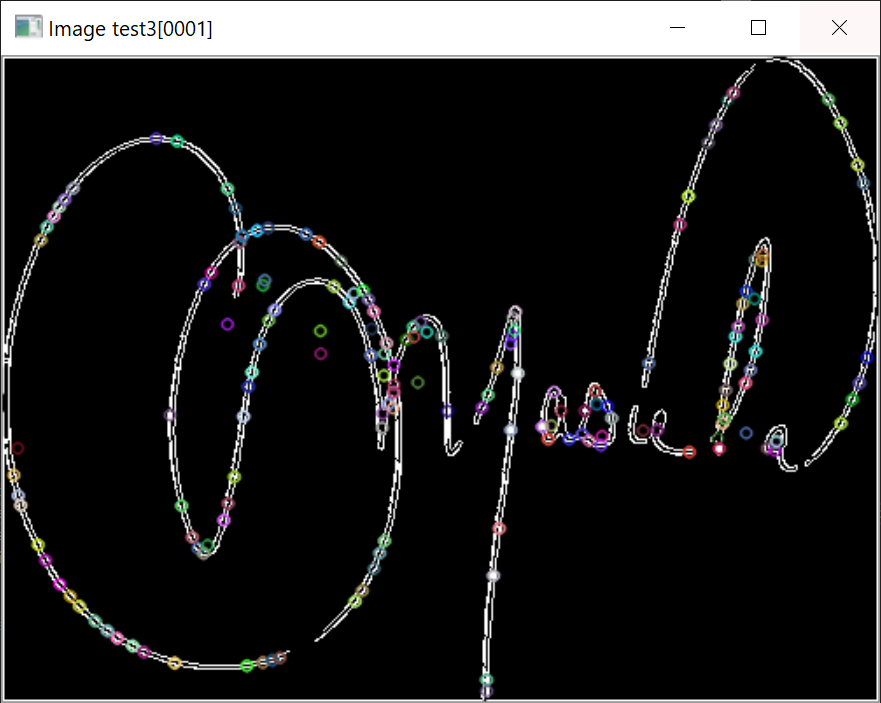
\includegraphics[scale=0.35]{Figures/DescriptoriSemnatura.PNG}
	\caption{Descriptori extrasi din semnatura}
	\label{fig:DescriptoriSemnatura}
\end{figure}

$\newline\newline$

Algoritmul k-means primeste ca valori de intrare o lista de puncte $X=\{x_{i},i=1:n\}$. Fiecare punct este d-dimensional $x_{i}=(x_{i1},x_{i2},...,x_{id})$. Obiectivul metodei k-means este gruparea punctelor în K multimi notate cu $S=\{S_{k}|k=1:K\}$. Centroidul care reprezinta submultimea k este notata cu $m_{k}$. Gruparea datelor trebuie realizata astfel incat sa fie minimizata functia obiectiv (Ecuatia \ref{eq:K-means}), unde $dist(.,.)$ reprezinta distanta Euclidiana in spatiul d-dimensional (Ecuatia \ref{eq:DistantaEuclidiana}).

\begin{equation} \label{eq:K-means}
J(X,S)=\sum_{k=1}^{K}\sum_{x\in S_{k}}dist(x,m_{k})
\end{equation}

In procesul algoritmului K-means se vor citi, decta si transforma imaginile de test, urmand ca apoi sa se genereze histogramele si antrenarea SVM. Rezultatul final este redat prin obtinerea valorii de 0\% sau 100\% a acuratetii clasificarii pentru fiecare categorie de test. Pentru fiecare proces este calculat timpul de executie in secunde. Un exemplu este prezentat in Tabelul \ref{RezultateKmeans}.

\begin{table}[h!]
	\caption{SET DE PROBABILITATI}
	\begin{center}
		\begin{tabular}{|c|c|}
			\hline
			\textbf{Categorii} & \textbf{Rezultat} \\
			\hline
			Categorie 1 de imagini de test & 0\% \\
			Categorie 2 de imagini de test & 100\% \\
			Categorie 3 de imagini de test & 0\% \\
			Categorie 4 de imagini de test & 0\% \\
			\hline
		\end{tabular}
		\label{RezultateKmeans}
	\end{center}
\end{table}

\section{Comparatie algoritmi utilizati}
Metoda de verificare a semnaturii prin compararea histogramei a numarului de pixeli de pe verticala si orizontala, folosind un numar redus de redus de acumulatoare, este utilizata pentru rezultate probabililistice pentru semnatura de intrare. Se obtine un procentaj pentru fiecare categorie parcursa in relatie cu imaginea de intrare. In schimb, algoritmul Kmeans este utilizat pentru rezultate mult mai precise pe baza antrenarii algoritmului cu imagini de test. Pe baza anumitor descriptori se creeaza un pattern, in urma careia se incadreaza imaginea intr-o anumita categorie.


\paragraph{Avantaje/Dezavantaje algoritm partitionare}
\begin{itemize}
	\item Cu cat numarul de acumulatoare este mai crescut, cu atat algoritmul de partitionare este mai precis in obtinerea rezultatelor.
	\item Prin introducere unei imagini ce nu face parte din nici o categorie, algortmul nu va incadra imaginea intr-o anumita categorie.
	\item Algoritmul este rapid in executie, iar datele sunt prezente imediat dupa parcurgerea unei categorii.
\end{itemize}

\paragraph{Avantaje/Dezavantaje algoritm Kmeans}
\begin{itemize}
	\item Algoritmul necesta un numar mare de imagini de test pentru o acuratete mai buna.
	\item Prin introducere unei imagini ce nu face parte din nici o categorie, algortmul este nevoit sa incadreze semnatura intr-o categorie cat mai apropiata de pattern-ul creat.
	\item Algoritmul necesita un timp de executie destul de mare pentru antrenare.
\end{itemize}


\section{Concluzii}
Acest document ofera o modalitate de verificare eficienta si simpla a unei semnaturii in mediul offline. Algoritmul a fost testat pe un set de semnaturi de test, iar rezultatele obtinute au fost in cea mai mare parte valide.

% Referinte
\begin{thebibliography}{00}
\bibitem{b1} Sikander Hans, Sachin Gupta, ``Algorithm For Signature Verification System'' Department of Electrical Instrumentation Engineering, Thapar University, Patiala, India, April 2012
\bibitem{b2} Mohan Mandaogade, Saurabh, Vishal Mhaske, ``Handwritten Signature Verification And Recognition Using ANN'', MPGI National Multi Conference 2012, 1892, 7-8 April 2012
\bibitem{b3} Radu Gabriel Danescu, ``Image Processing``, Laboratory 11: Edge detection
\bibitem{b4} Costin-Gabriel Chiru, Stefan Trausan-Matu, Traian Rebedea, ``O imbunatatire a performantelor algoritmului KNN in sistemele de recomandare pe web'' Interactiune Om-Calculator, Universitatea Politehnica Bucuresti , 2008
\bibitem{b5} P.A.Charde, S.D.Lokhande, ``Classification Using K Nearest Neighbor for Brain
Image Retrieval'', International Journal of Scientific $\&$ Engineering Research, Volume 4, Issue 8, August-2013, 760-765, ISSN 2229-5518
\bibitem{b6} Isha, Pooja, Varsha, ``Offline Signature Verification based on Euclidean distance using Support Vector Machine'', International Journal of Advanced Engineering, Management and Science (IJAEMS), Vol-2, Issue-8, Aug-2016, ISSN: 2454-1311
\bibitem{b7} Richard Szeliski, ``Computer Vision: Algorithms and Applications'', September 3, 2010, Chapter 5.3.1 ``K-means and mixtures of Gaussians'' pages 289-292, Chapter 14.4.1 ``Bag of words'' pages 697-701
\bibitem{b8} J. A. Hartigan and M. A. Wong, ``Algorithm AS 136: A K-Means Clustering Algorithm'', Vol. 28, No. 1 (1979), pages 100-108
\bibitem{b9} ``DescriptorMatcher::match'', website: https://docs.opencv.org/2.4/modul es/features2d/doc/common\_interfaces\_of\_descriptor\_matchers.html
\end{thebibliography}
\vspace{12pt}

\end{document}
